\documentclass[12pt, a4paper]{article}
\usepackage[francais]{babel}
\usepackage{caption}
\usepackage{graphicx}
\usepackage[T1]{fontenc}
\usepackage{listings}
\usepackage{geometry}
\usepackage{minted}
\usepackage{array,multirow,makecell}
\usepackage{float}
\usepackage[colorlinks=true,linkcolor=black,anchorcolor=black,citecolor=black,filecolor=black,menucolor=black,runcolor=black,urlcolor=black]{hyperref}
\setcellgapes{1pt}
\makegapedcells
\usepackage{fancyhdr}
\pagestyle{fancy}
\lhead{}
\rhead{}
\chead{}
\rfoot{\thepage}
\lfoot{Baumgaertner - Rehm - Doghmane}
\cfoot{}
\renewcommand{\footrulewidth}{0.4pt}
\renewcommand{\headrulewidth}{0.4pt}
\renewcommand{\listingscaption}{Code}
\renewcommand{\listoflistingscaption}{Table des codes}

% \usepackage{mathpazo} --> Police à utiliser lors de rapports plus sérieux

\begin{document}
\begin{titlepage}
	\newcommand{\HRule}{\rule{\linewidth}{0.5mm}} 
	\center 
	\textsc{\LARGE iut de colmar}\\[4.5cm] 
	\textsc{\Large SAE 24}\\[0.5cm] 
	\textsc{\large projet intégratif}\\[0.5cm]
	\HRule\\[0.75cm]
	{\huge\bfseries Partie téléphonie}\\[0.4cm]
	\HRule\\[1.5cm]

	% Utiliser les lignes qui suivent dans le cas où il y a plusieurs membres
	%------------------------------------
	\begin{minipage}{0.4\textwidth}
		\begin{flushleft}
			\large
			\textit{RT11}\\
			Martin \textsc{Baumgaertner}
		\end{flushleft}
	\end{minipage}
	~
	\begin{minipage}{0.4\textwidth}
		\begin{flushright}
			\large
			\textit{RT12}\\
			Mehdi \textsc{Rehm}
		\end{flushright}
	\end{minipage}
    \\[0.7cm]
    \begin{minipage}{0.4\textwidth}
		\begin{flushleft}
			\large
			\textit{RT11}\\
			Sâji \textsc{Doghmane}
		\end{flushleft}
	\end{minipage}
	~
    \begin{minipage}{0.4\textwidth}
		\begin{flushright}
			\large
			\textit{\textcolor{white}{Mehdi}}\\
			\textcolor{white}{Mehdi} \textsc{\textcolor{white}{Mehdi}}
		\end{flushright}
	\end{minipage}
    
	%------------------------------------
    %------------------------------------
	% \textsc{\large martin baumgaertner}\\[0.5cm] % S'il y que moi qui écrit
    %------------------------------------
	\vfill\vfill\vfill
	{\large\today} 
	\vfill
\end{titlepage}
\newpage
\tableofcontents
\newpage
\listoffigures
\newpage



\newpage
\section{Cahier des charges}

Le réseau à intégrer est le suivant : 1 poste IP, 1 poste numérique et 1 poste analogique.
Ces équipements seront intégrés au VLAN VoIP.
Un trunk SIP devra être mis en place afin d’effectuer des appels vers le réseau téléphonique publique.
Les caractéristiques sont les suivantes :\\

	\begin{itemize}
		\item @IP du serveur = 10.129.10.20
		\item @IP du registrar = 10.129.10.20
		\item Nom de compte = table6
		\item Login = table6
		\item Mot de passe = toto
		\item SDA = 09.89.20.6.xxx
	\end{itemize}

	\begin{figure}[H]
		\centering
		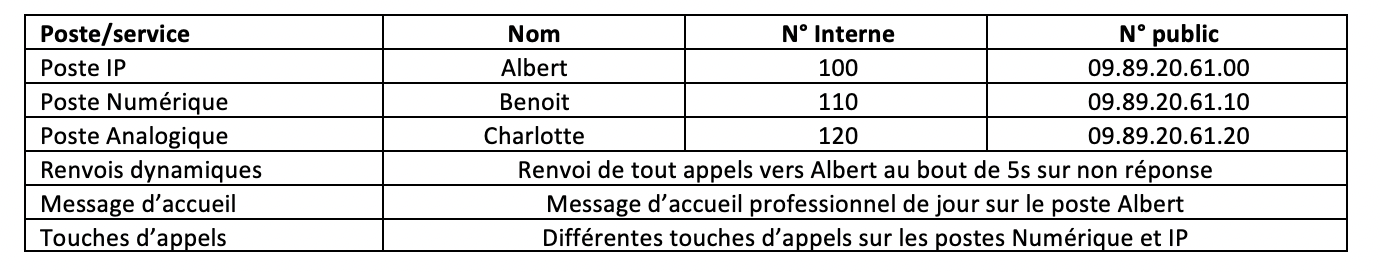
\includegraphics[width=1\textwidth]{img/tableau.png}
		\caption{Tableau résumant les tâches à réaliser}
		\label{fig:ch}
	\end{figure}

\section{Préliminaires}

	\subsection{Installation du matériel}

	Voici, ci après le schéma d'installation à réaliser :
	\begin{figure}[H]
		\centering
		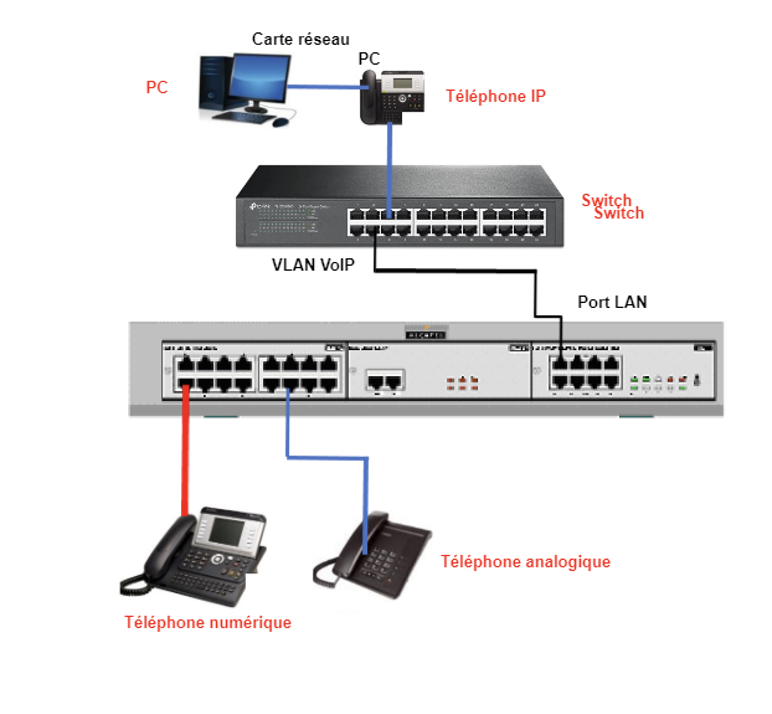
\includegraphics[width=0.3\textwidth]{img/schema.png}
		\caption{Schéma d'installation}
		\label{fig:sh}
	\end{figure}
	

	\subsection{Démarrage et connexion au PABX}

	Afin de se connecter au PABX il faut changer l’adresse IP de la carte réseau du PC
	pour être dans le même réseau que le PABX. Pour changer l’adresse IP de la carte réseau 
	du PC, il faut aller dans « Modifier les options d’adaptateur » dans « Paramètres réseau 
	avancés » puis on sélectionne la carte réseau à paramétrer, on fait un clic droit puis 
	« Paramètre » -> « Protocole Internet version 4 » et on peut réaliser la modification.
	Lorsqu’on est maintenant dans le même réseau, on peut lancer le logiciel « OMC 920 23.1a » 
	puis on se connecte ensuite au mode « Expert ».

	\begin{figure}[H]
		\centering
		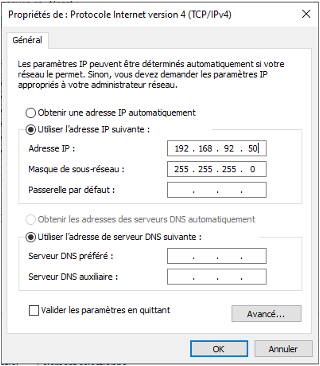
\includegraphics[width=0.4\textwidth]{img/co.png}
		\caption{Configuration IP de la machine}
		\label{fig:co}
	\end{figure}

	Après avoir choisi ce mode, on ouvre le menu « Communication » -> « Connecter ».
	Lorsqu’on est arrivé dans le menu « Mode de communication », on a automatiquement
	l’adresse par défaut du PABX et on peut se connecter en cliquant sur « OK », le mot 
	de passe est : « pbxk1064 ».
	\newpage

\section{Configuration du matériel}

	\subsection{Configuration IP du PABX}

	Pour la configuration IP du PABX, il faut que le PABX soit dans le VLAN10 « Voix ». 
	L’adresse réseau de ce VLAN est la suivante : « 172.114.10.0 ». Il faudra donc adapter 
	la configuration, il faut aller dans le menu « Matériels et Limites » puis « Configuration 
	LAN / IP ». Plusieurs configurations sont à réaliser, voici les configurations :

	\begin{figure}[h]
		\begin{minipage}[c]{.46\linewidth}
			\centering
			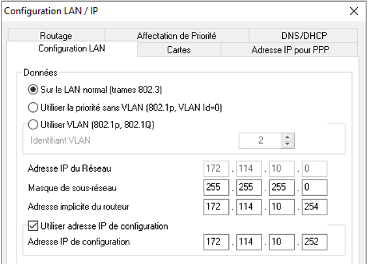
\includegraphics{img/lan.png}
			\caption{Configuration du LAN}
		\end{minipage}
		\hfill%
		\begin{minipage}[c]{.46\linewidth}
			\centering
			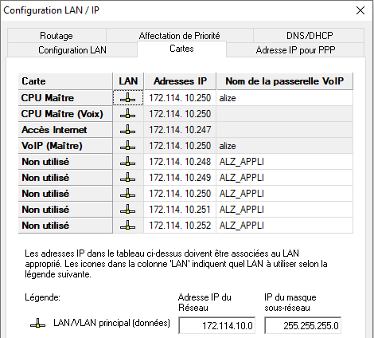
\includegraphics{img/carte.png}
			\caption{Configuration de la carte}
		\end{minipage}
	\end{figure}

	\begin{figure}[H]
		\centering
		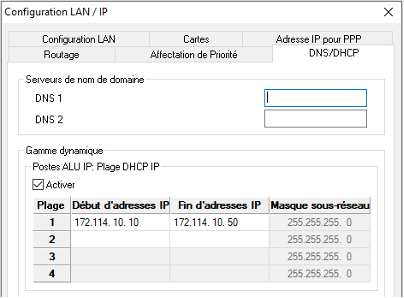
\includegraphics[width=0.7\textwidth]{img/dhcp.png}
		\caption{Configuration du DHCP}
		\label{fig:dhcp}
	\end{figure}

	Nous avons donc configuré le LAN (adresse IP réseau, masque, passerelle …), 
	la configuration de la carte (adresse IP du PABX « CPU Maître ») et le DHCP 
	(plage d’adresse IP). Lorsqu’on a fini la configuration IP, le logiciel redémarre 
	puis on peut brancher notre PABX au VLAN « Voix » et on se reconnecte avec la 
	nouvelle adresse IP du PABX.

	\subsection{Configuration Voix sur IP}

	Suite à la reconnexion au PABX, nous allons effectuer la configuration VoIP. 
	Il faut aller dans le menu « Voix sur IP » puis « VoIP : Paramètres ». Deux 
	configurations sont à réaliser, voici les configurations :

	\begin{figure}[h]
		\begin{minipage}[c]{.46\linewidth}
			\centering
			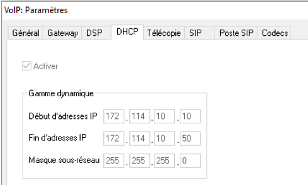
\includegraphics{img/menudh.png}
			\caption{Menu DHCP}
		\end{minipage}
		\hfill%
		\begin{minipage}[c]{.46\linewidth}
			\centering
			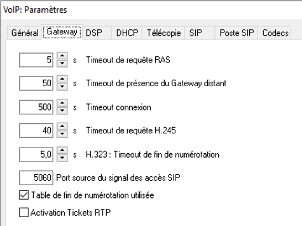
\includegraphics{img/gate.png}
			\caption{Mneu gateway}
		\end{minipage}
	\end{figure}

	Pour le DHCP, on affecte une plage d’adresse IP au téléphone présent dans notre réseau.
	La plage est la suivante : 172.114.10.10 à 50. Suite à cela le téléphone IP aura une 
	adresse automatique attribuée.
	
	\newpage
	\subsection{Configuration des téléphones}

	Nous allons maintenant effectuer la configuration des différents postes du réseau, 
	il faut se rendre dans le menu « Liste des Postes/Bornes ». Pour modifier un poste, 
	il faut sélectionner un poste puis on renseigne un numéro d’annuaire, un nom et enfin 
	on clique sur modifier.

	\begin{figure}[H]
		\centering
		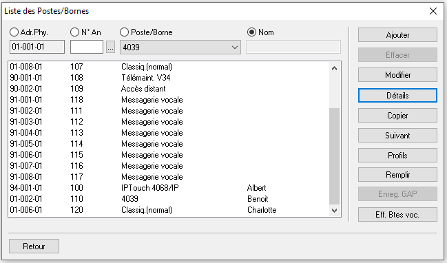
\includegraphics[width=0.8\textwidth]{img/liste.png}
		\caption{Liste postes/bornes}
		\label{fig:liste}
	\end{figure}

	On peut effectuer un test en appelant les téléphones par leurs numéros interne 
	afin de savoir si la configuration fonctionne.

\section{Mise en place du trunk SIP}

Afin d’effectuer des appels vers le réseau téléphonique publique, nous allons
mettre en place un trunk SIP. On va tout d’abord ouvrir l’accès VoIP pour le PABX,
afin d’effectuer cette tâche, il faut se rendre dans le menu « Voix sur IP » puis « VoIP :
Paramètres ».

\begin{figure}[H]
	\centering
	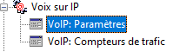
\includegraphics[width=0.4\textwidth]{img/menuv.png}
	\caption{Menu Voix sur IP}
	\label{fig:menuv}
\end{figure}
\newpage

Dans le menu « Voix sur IP » -> « Général », on modifie le nombre de canaux accès VoIP à 2.

\begin{figure}[H]
	\centering
	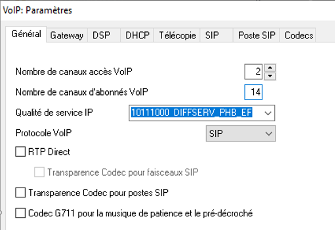
\includegraphics[width=0.6\textwidth]{img/menug.png}
	\caption{Menu général}
	\label{fig:menug}
\end{figure}

Dans le menu « Gateway », on coche la case « Table de fin de numérotation utilisée ».

\begin{figure}[H]
	\centering
	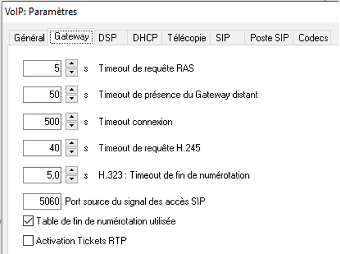
\includegraphics[width=0.6\textwidth]{img/mg.png}
	\caption{Menu gateway}
	\label{fig:mg}
\end{figure}

Afin de vérifier l’apparition et la présence de notre accès externe, on se rend dans le
menu « Lignes Externes » -> « Tableau des accès externes ». On peut remarquer que nos accès
sont bien présents.

\begin{figure}[h]
	\begin{minipage}[c]{.46\linewidth}
		\centering
		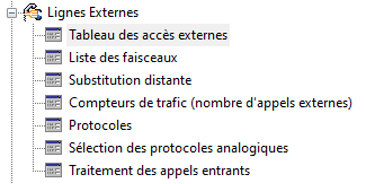
\includegraphics{img/ligne.png}
		\caption{Menu lignes externes}
	\end{minipage}
	\hfill%
	\begin{minipage}[c]{.46\linewidth}
		\centering
		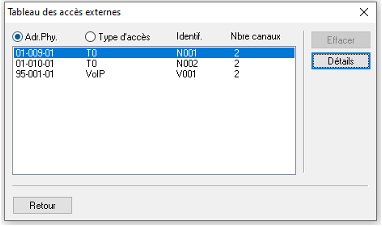
\includegraphics{img/mt.png}
		\caption{Menu tableau des accès externes}
	\end{minipage}
\end{figure}

Pour finir on va configurer le faisceau principal, pour cela on se rend dans le menu
« Lignes Externes » -> « Liste des faisceaux ». On supprime les faisceaux pour laisser
ensuite le faisceau VoIP dans notre accès VoIP.

\begin{figure}[H]
	\centering
	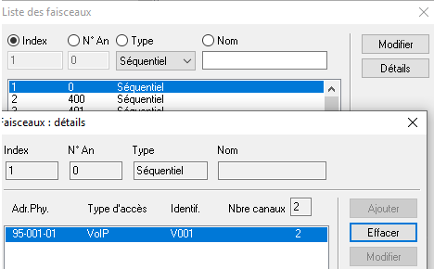
\includegraphics[width=0.6\textwidth]{img/fs.png}
	\caption{Liste des faisceaux}
	\label{fig:fs}
\end{figure}

Dans les détails de notre accès VoIP, on doit cliquer sur « Catégories de liaison ».
Puis on remplace 1 à CL3 et 2 à CL2. Ce sont des règles qu’on a mis sur ce faisceau VoIP. \\

\begin{itemize}
	\item CL3 = 1
	\item CL2 (Voix) = 2
\end{itemize}

\begin{figure}[H]
	\centering
	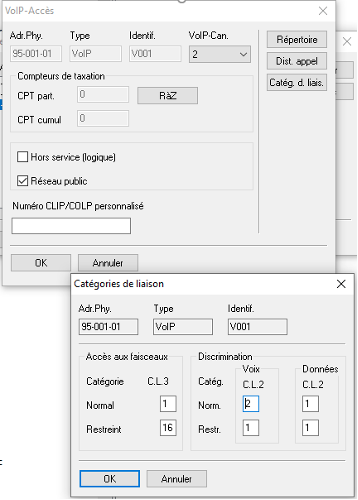
\includegraphics[width=0.4\textwidth]{img/fsd.png}
	\caption{Liste des faisceaux - détails}
	\label{fig:fsd}
\end{figure}

\section{Configurations diverses}

	\subsection{Plan de numérotation}

	On va maintenant acheminer le faisceau principal vers la table ADL, pour
	cela on se rend dans « Plans de numérotation » et « Plan de numérotation interne ».
	On va modifiez la ligne « Faisceau principal » en gardant le préfixe « 0 » comme prise
	du faisceau principal mais celui-ci est dirigé vers la table ADL public en étant absorbé.

	\begin{figure}[H]
		\centering
		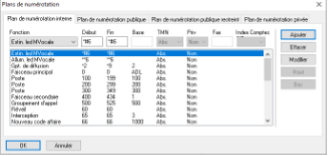
\includegraphics[width=0.6\textwidth]{img/interne.png}
		\caption{Plans de numérotation interne}
		\label{fig:interne}
	\end{figure}

	\newpage

	Lorsqu’on a fini le plan de numérotation interne, on modifie ensuite le plan de
	numérotation publique dans le même menu mais dans la partie « Plan de numérotation
	publique ». Je renseigne mes numéros internes.

	\begin{figure}[H]
		\centering
		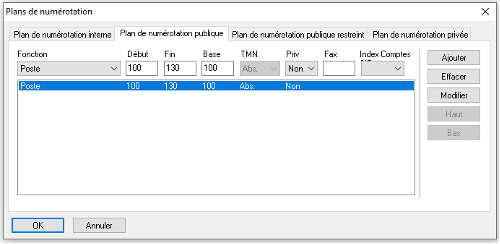
\includegraphics[width=0.6\textwidth]{img/publique.png}
		\caption{Plans de numérotation publique}
		\label{fig:publique}
	\end{figure}

	On va modifier ensuite la table de modification de numéros SDA dans le menu
	« Table de modification de numéros SDA » dans le menu « Plan de numérotation »,
	les numéros fournis par le simulateur sur le trunk SIP sont les suivants : 09 89 20 6xxx.

	\begin{figure}[H]
		\centering
		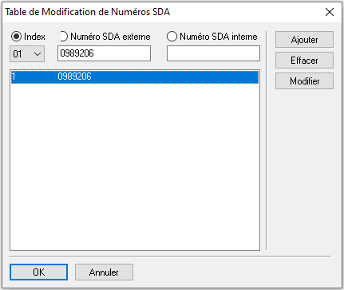
\includegraphics[width=0.6\textwidth]{img/msda.png}
		\caption{Modification des numéros SDA}
		\label{fig:msda}
	\end{figure}

	\newpage

	Dans le répertoire ADL « Plan de numérotation » -> « Appel direction logique » ->
	« Compte SIP », afin de créer un compte SIP avec le login et le mot de passe.
	Cela va nous permettre de nous authentifier sur le serveur VoIP. Le serveur enregistra
	le compte pour pouvoir fournir le service SIP et les numéros SDA.

	\begin{figure}[H]
		\centering
		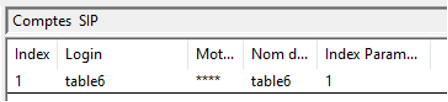
\includegraphics[width=0.6\textwidth]{img/sip.png}
		\caption{Compte SIP}
		\label{fig:sip}
	\end{figure}

	Dans le menu « Tableau ADL » du répertoire « Appel direction logique »,
	on configure les champs comme suit : 

	\begin{figure}[H]
		\centering
		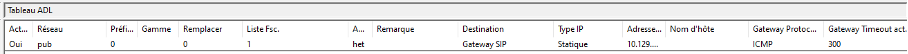
\includegraphics[width=1\textwidth]{img/adl.png}
		\caption{Tableau ADL}
		\label{fig:adl}
	\end{figure}

	Suite à la création du SIP, on va configurer la Gateway SIP su répertoire ADL
	dans le menu « Paramètre de Gateway ». Voici la configuration :

	\begin{figure}[H]
		\centering
		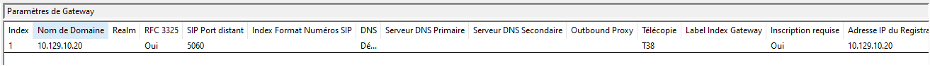
\includegraphics[width=1\textwidth]{img/paragate.png}
		\caption{Paramètres de Gateway}
		\label{fig:paragate}
	\end{figure}

	Dans liste des faisceaux, on va configurer la « Listes des Faisceaux » comme
	sortie la n°1 de la table ADL, voici la configuration ci-dessous.

	\begin{figure}[H]
		\centering
		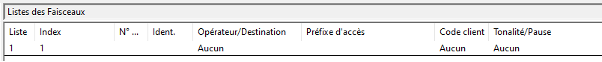
\includegraphics[width=1\textwidth]{img/listefs.png}
		\caption{Liste des faisceaux}
		\label{fig:listefs}
	\end{figure}
	\newpage
	\subsection{Numérotation par blocs}

	Les postes numériques et analogiques ne peuvent pas composer de numéros sur
	l’opérateur Astérisk, il ne comprend pas la numérotation par chevauchement. Il comprend
	que la numérotation par bloc. Afin de résoudre ce problème, il faut forcer le PABX à ne
	faire que de la numérotation par bloc. Pour cela, il faut ouvrit le menu « Particularité
	Système » -> « Lecture/Ecriture » -> « Mémoire » -> « Tempo : Adresses par libellé ».
	Dans la ligne « IsdnblkTim », on clique sur « Détails » puis on modifie la valeur à
	« 00 3E ». 

	\begin{figure}[H]
		\centering
		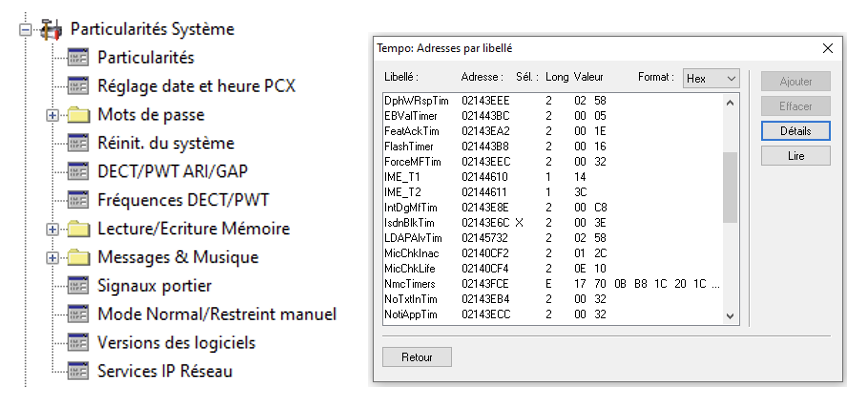
\includegraphics[width=0.5\textwidth]{img/bloc.png}
		\caption{Numérotation par bloc}
		\label{fig:bloc}
	\end{figure}

	\subsection{Renvois dynamiques}

	Pour le renvoi dynamique, nous allons configurer le renvoie sur le téléphone
	« Benoit » et « Charlotte ». Dans « Liste des Postes/Bornes », on sélectionne
	les deux téléphones puis « Détail » et dans « Renvois dynamiques » et on remplit
	les éléments suivants :

	\begin{figure}[H]
		\centering
		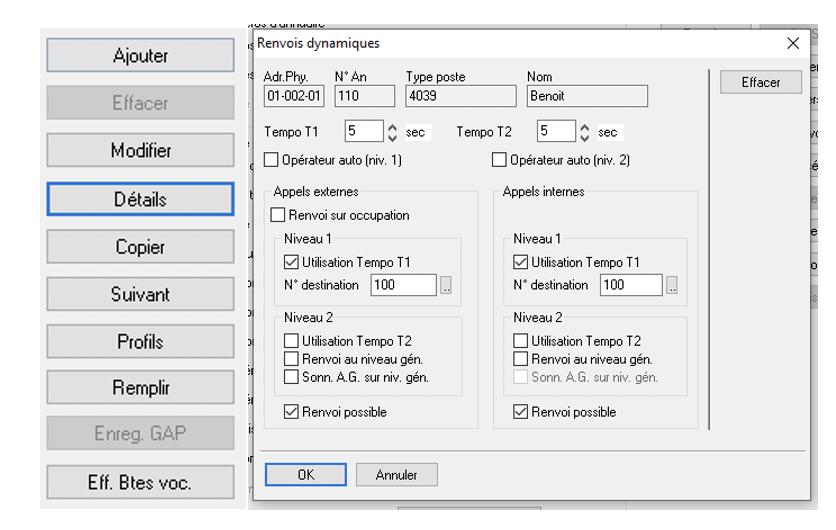
\includegraphics[width=0.5\textwidth]{img/nbloc.png}
		\caption{Renvois dynamiques}
		\label{fig:nbloc}
	\end{figure}

	\subsection{Message d'accueil}

	Dans l’écran d’accueil du téléphone IP, on choisit le menu "IntApp" -> "Opérat".
	On entre le mot de passe "help1954" , puis on choisit le menu "Avancé" -> "Voix" ->
	"MGarde". Pour enregistrer un message, on choisit "Enreg" -> "Enreg", lorsqu’on a
	fini notre message on sélectionne "STOP" puis "OK". On va maintenant configurer le
	"Prédécroché" dans le menu "Particularités postes" -> "Prédécroché". Dans
	"Prédécroché", dans "Pub" on sélectionne les 2 petits points "..", et on prend le
	téléphone de "Albert". On clique ensuite sur "Détails", et je remplis les informations
	suivantes ci-dessous et je copie-coller pour chaque jour de la semaine.

	\begin{figure}[H]
		\centering
		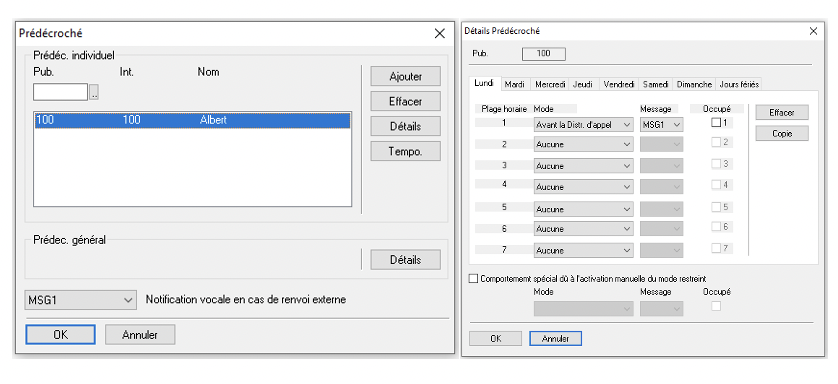
\includegraphics[width=0.5\textwidth]{img/pd.png}
		\caption{Prédécroché et détails}
		\label{fig:pd}
	\end{figure}


	\subsection{Touches d'appels}

	Pour mettre des touches d’appel sur les téléphones, on se rend dans « Liste des
	postes/bornes », on sélectionne un poste téléphonique dans laquelle on va attribuer
	des touches. Puis dans « Touches » et on remplit les informations suivantes :

	\begin{figure}[H]
		\centering
		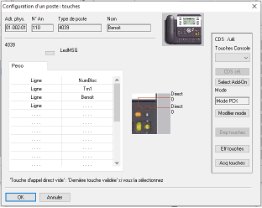
\includegraphics[width=0.5\textwidth]{img/ctou.png}
		\caption{Configuration des touches}
		\label{fig:ctou}
	\end{figure}

	\subsection{Groupement}

	Pour réaliser un groupement, on se rend dans « Liste des groupements d’appel »,
	on remplit le type en « Parallèle » et le nom du groupe « GROUPE » par exemple.

	\begin{figure}[H]
		\centering
		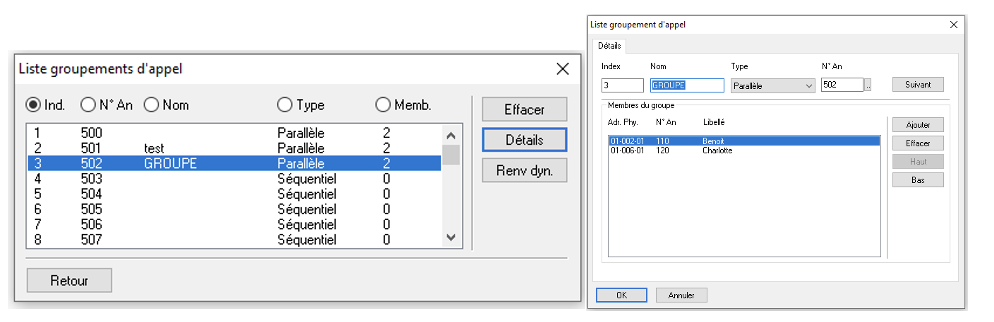
\includegraphics[width=0.9\textwidth]{img/grp.png}
		\caption{Groupement}
		\label{fig:grp}
	\end{figure}

\section{Conclusion}

Cet exercice de téléphonie nous aura permis de consolider les bases de la téléphonie d'entreprise
et nous aura appris beaucoup de choses sur le travail en autonomie. Sans aide des professeurs, 
nous étions livrés fasse à nous mêmes, et c'est plutôt un bon exercice. Ça permet de voir que
finalement, nous sommes toujours (dans la plupart des situations) capables de trouver tout seuls
une solution à nos problèmes.

\end{document}